\part{Esercizi}
\section{Introduzione}
Per una maggior comprensione è giusto mostrare degli esercizi svolto e visto che ci sono alcuni casi in cui serve fare ulteriori operazioni per risolvere lo studio\dots

\chapter{Soluzioni}
\section {Infinitesimi e infiniti}
\subsection{Esercitazione 1}
\begin{equation}
	y=1-\sqrt{1+x}
\end{equation}
\begin{equation*}
	\lim_{x\to0}\left[\frac{1-\sqrt{1+x}}{\sqrt{x}}\right]=\lim_{x\to0}\frac{\frac{1}{2\sqrt{1+x}}}{\frac{1}{2\sqrt{x}}}=-\frac{1}{\not{2}\sqrt{1+x}}*\not{2}\sqrt{x}=\frac{0}{1}=0
\end{equation*}
da questo si deduce che il limite non è di ordine $\frac{1}{2}$ come ipotizzato inizialmente ma risulta di un ordine maggiore, allora il passo successivo è tentare con l'ordine 1:
\begin{equation*}
	\lim_{x\to0}\left[\frac{1-\sqrt{1+x}}{x}\right]=\lim_{x\to0}-\frac{1}{2\sqrt{1+x}}=-\frac{1}{2}
\end{equation*}
e appunto in questo caso $ord\left(1-\sqrt{1+x}\right)=1$
\subsection{Esercitazione 2}
\begin{equation}
	f(x)=(1+x)^2-1
\end{equation}
\begin{equation*}
	\lim_{x\to0}\frac{(1+x)^2-1}{x}=\lim_{x\to0}2(1+x)=2
\end{equation*}
Da questo si evince che $ord\left[(1+x)^2-1\right]=1$, quindi è un infinitesimo di ordine 1.
\subsection{Esercitazione 3}
\begin{equation}
	f(x)=\tan x
\end{equation}
\paragraph{Ipotesi:} $\lim\limits_{x\to0}\tan x$ è di ordine 1
\begin{equation}
	\lim_{x\to0}\frac{\tan x}{x}=\lim_{x\to0}\frac{\frac{1}{\cos^2x}*x-\tan x*1}{x^2}=\lim_{x\to0}\frac{\frac{x}{\cos^2x}-\tan x}{x^2}=\lim_{x\to0}\frac{\frac{x-\tan x \cos^2x}{\cos^2x}}{x^2}=\frac{x-\tan x \cos^2x}{\cos^2x}*x^2=
\end{equation}

\section{Studio di funzione}
\subsection{Esercitazione 1}
\begin{equation}
	f(x)=\ln\left(x-x^3\right)
\end{equation}
\begin{enumerate}
	\item Dominio
	\begin{equation*}
		x-x^3>0
	\end{equation*}
	
	Per procedere dobbiamo raggruppare, mettendo come valor comune la $x$
	\begin{equation*}
		x(1-x^3)>0
	\end{equation*}
	Quindi prendiamo i due casi singolarmente e il risultato sarà $x>0$ e $x<\pm1$, quindi il dominio sarà
	\begin{equation*}
		\forall x\in (-\infty,-1) \vee (0,1)
	\end{equation*}
	\item Intersezione con l'asse x
		\begin{equation*}
			\begin{matrix}
				\ln\left(x-x^3\right)=0\\
				x-x^3=1\\
				-x^3+x-1=0
			\end{matrix}
		\end{equation*}
	\item comportamento agli estremi del dominio
		\begin{equation*}
			\lim_{x\to -\infty}\ln\left(x-x^3\right)=-\infty+\infty
		\end{equation*}
		in questo caso non può essere utilizzata la regola di De l'Hopital per risolvere la forma indeterminata, quindi il metodo più semplice è quello di mettere in evidenza la x e procedere.
		
	\item Derivata prima
	\begin{equation*}
		f^\prime(x)=\frac{1}{(x-x^3)}\left(1-3x^2\right)=\frac{1-3x^2}{x-x^3}
	\end{equation*}
	Andremo a studiare solo il numeratore perché il denominatore è già stato definito nel dominio, quindi è l'unica cosa che può identificare il segno e quindi l'andamento della funzione.
	\begin{equation}
		\begin{matrix}
			1-3x^2=0\\
			-3x^2=-1\\
			3x^2=1\\
			x^2=\frac{1}{3}\\
			x=\pm\sqrt{\frac{1}{3}}=\pm\frac{1}{\sqrt{3}}
		\end{matrix}
	\end{equation}
	In questo caso è presente un punto di massimo e quindi dobbiamo calcolarlo per poterlo tracciare nel disegno.
	\begin{equation*}
		f\left(\frac{1}{\sqrt{3}}\right)=\ln\left(\frac{1}{\sqrt{3}}-\frac{1}{3\sqrt{3}}\right)=\ln\left(\frac{3-1}{3\sqrt{3}}\right)=\ln\left(\frac{2}{3\sqrt{3}}\right)
	\end{equation*}
	Quindi il massimo si trova in $\max\left[\frac{1}{\sqrt{3}}; \ln\left(\frac{2}{3\sqrt{3}} \right) \right]$
	\item grafico
	\begin{figure}[!ht]
		\centering
		\begin{tikzpicture}
			\node[] (pic) at (0,0) {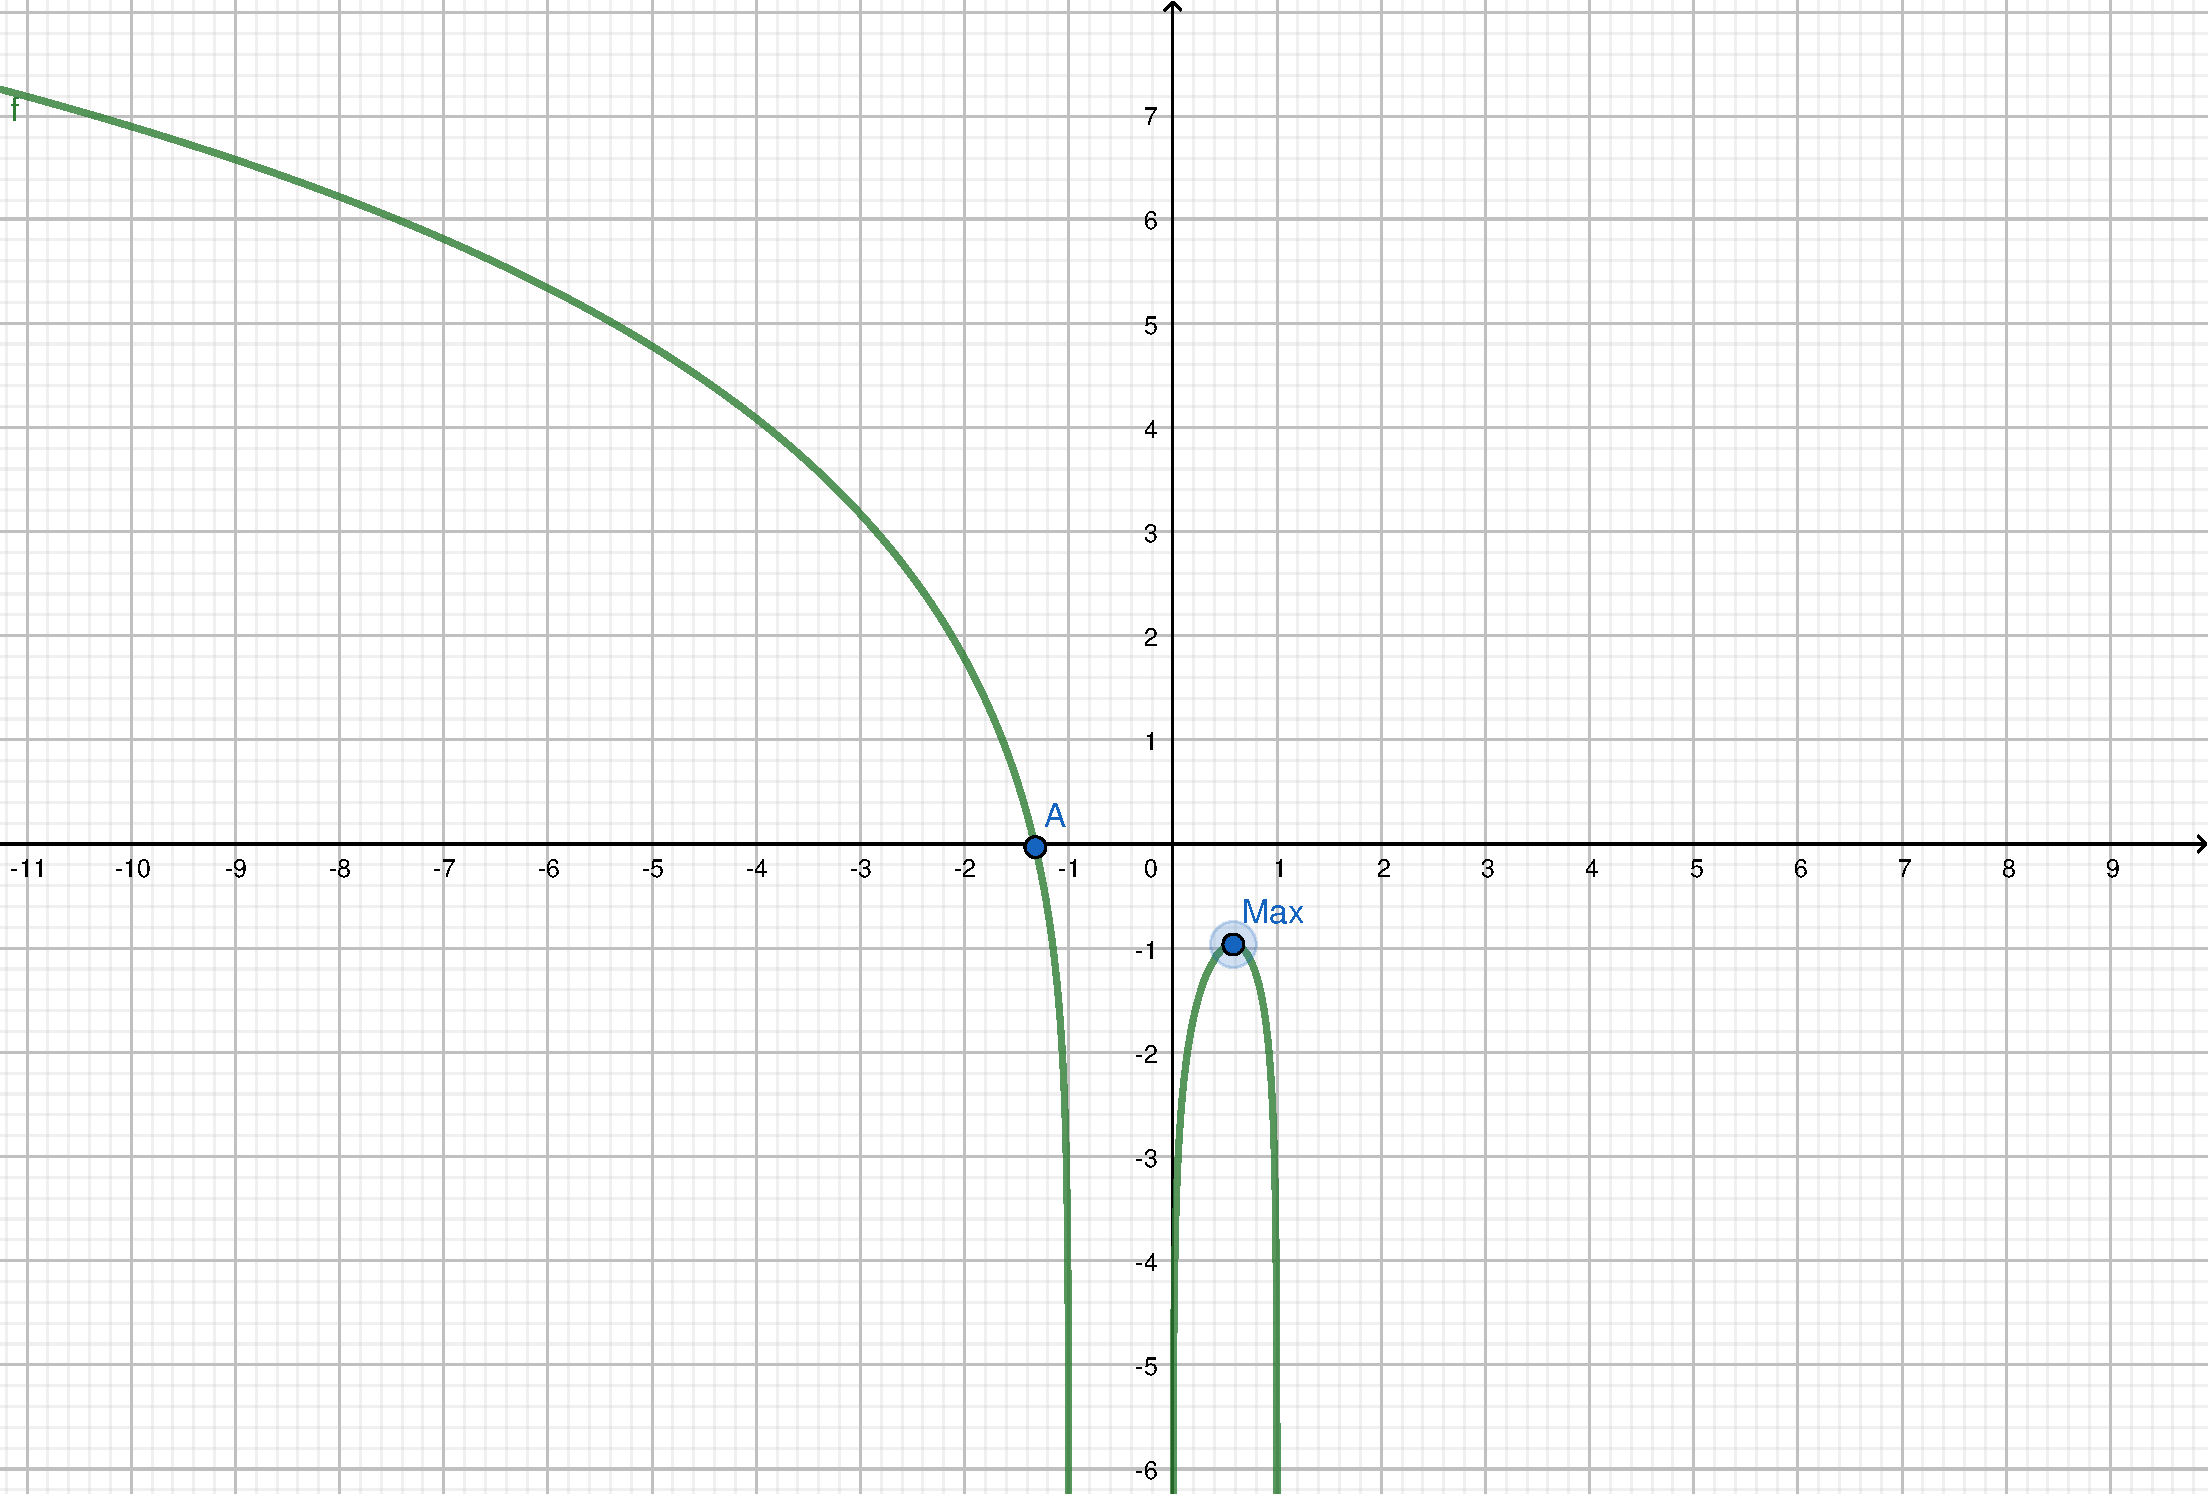
\includegraphics[height=8cm]{img/esercitazioni/esercitazione 1.pdf}};
		\end{tikzpicture}
		\caption{Grafico di Funzione $f(x)=\ln\left(x-x^3\right)$}
	\end{figure}
\end{enumerate}\newpage
\section{Integrali indefiniti}
\subsection{esercitazione 1}
	\begin{equation}
		\begin{matrix}
			\int e^{-3x}dx=-\frac{1}{3}e^{-3x}+C \\
			F(x)=-\frac{1}{3}e^{-3x}+C \\
			f(x)=e^{-3x}\\
			F^\prime(x)=-\frac{1}{3}*e^{-3x}*(-3)=e^{-3x}=f(x)
		\end{matrix}
	\end{equation}
\subsection{esercitazione 2}
	\begin{equation}
		\begin{matrix}
			\int x*e^{2x}dx\\
			\frac{1}{2}e^{2x}*x-\int\frac{1}{2}e^{2x}*1dx\\
			\frac{1}{2}e^{2x}*x-\frac{1}{2}\inf e^{2x}dx \\
			\frac{1}{2}e^{2x}*x-\frac{1}{2}*\frac{1}{2}e^{2x}+C\\
			\frac{1}{2}e^{2x}*\left( x-\frac{1}{2}\right)+C
		\end{matrix}
	\end{equation}
\subsection{esercitazione 3}
	\begin{equation}
		\begin{matrix}
			\int x^2dx=\frac{1}{3}x^3+C\\
			f(x)=x^2\\
			F(x)=\frac{1}{3}x^3+C\\
			D\left(\frac{1}{3}x^3+C\right)=\frac{1}{3}*3x^2=x^2
		\end{matrix}
	\end{equation}
\subsection{esercitazione 4}
	\begin{equation}
		\begin{matrix}
			\int \frac{1}{x}dx=\ln\left|x\right|+C\\
			\text{Dimostrazione}\\
			\ln\left|x\right|=\begin{cases}
					\ln x & \text{ se x > 0}\\
					\ln -x & \text{ se x < 0}
			\end{cases}\\
			D\ln\left|x\right|=\begin{cases}
				\frac{1}{x}\\
				\frac{1}{-x}*(-1)=\frac{1}{x}
			\end{cases}
		\end{matrix}
	\end{equation}
\subsection{esercitazione 5}
	\begin{equation}
		\begin{matrix}
			\int \frac{2x}{x^2+5}dx=\ln\left|x^2+5\right|+C
		\end{matrix}
	\end{equation}
\subsection{esercitazione 6}
	\begin{equation}
		\begin{matrix}
			\int \frac{3x^2}{x^2+1}dx=\ln\left|x^2+5\right|+C
		\end{matrix}
	\end{equation}
\subsection{esercitazione 7}
	\begin{equation}
		\begin{matrix}
			\int \frac{1}{y}dx=\ln y+C\\
			=\int \frac{1}{y^3}dy=\int y^{-3}dx\\
			=\int \frac{1}{-3+1}y^{-3+1}+C\\
			=-\frac{1}{2}y^{-2}+C\\
			=-\frac{1}{2y^2}+C
		\end{matrix}
	\end{equation}
\subsection{esercitazione 8}
	\begin{equation}
		\begin{matrix}
			\int \frac{1}{\sqrt{y}}dy\\
			\int
			y^{\frac{1}{2}}dy=\frac{1}{-\frac{1}{2}+1}y^{-\frac{1}{2}+1}+C\\
			=\frac{1}{\frac{1}{2}}y^\frac{1}{2}+C=2\sqrt{y}+C
		\end{matrix}
	\end{equation}
\subsection{esercitazione 9}
	\begin{equation}
		\begin{matrix}
			\int \frac{1}{\sqrt[3]{y}}dy=\int y^{-\frac{1}{3}}dy\\
			=\frac{1}{-\frac{1}{3}+1}y^{\frac{1}{3}+1}+C\\
			=\frac{1}{\frac{2}{3}}*y^{\frac{2}{3}}+C\\
			=\frac{3}{2}\sqrt[3]{y^2}+C\\
			-\frac{1}{3}+1=\frac{-1+3}{3}=\frac{2}{3}
		\end{matrix}
	\end{equation}
\subsection{esercitazione 10}
	\begin{equation}
		\begin{matrix}
			\int \sqrt[3]{y^2}dy=\int y^{\frac{2}{3}}dy\\
			=\frac{1}{\frac{2}{3}+1}y^{\frac{2}{3}+1}dy\\
			=\frac{1}{\frac{2+3}{3}}y^{\frac{2+3}{3}}dy\\
			=\frac{1}{\frac{5}{3}}y^{\frac{5}{3}}\\
			=\frac{3}{5}y^\frac{5}{3}\\
			=\frac{3}{5}\sqrt[3]{y^5}
		\end{matrix}
	\end{equation}
\subsection{esercitazione 11}
	\begin{equation}
		\begin{matrix}
			\int \sqrt[3]{y^2}\,dy=\int
			y^{\frac{2}{3}}dy\\
			=\frac{1}{\frac{2}{3}+1}y^{\frac{2}{3}+1}dy+C\\
			=\frac{1}{\frac{5}{3}}y^{\frac{5}{3}}+C\\
			=\frac{3}{5}\sqrt[3]{y^5}+C
		\end{matrix}
	\end{equation}
\section{Integrali definiti}
\subsection{Esercitazione 1}
	\begin{equation}
		\begin{matrix}
			\int_{1}^{3} \frac{x+1}{x+2}\,dx\\
			\left[x-\ln\abs{x+2}\right]_{1}^{3}\\
			=[3-\ln 5]-[1-\ln 3]\\
			=3-\ln 5-1+\ln 3\\
			=2+\ln\frac{3}{5}
		\end{matrix}
	\end{equation}
\subsection{Esercitazione 2}
	\begin{equation}
		\begin{matrix}
			\int_{1}^{3} \frac{x+1}{x+2}\,dx\\
			\int \frac{x+1+1-1{x+2}}\,dx\\
			=\int \frac{(x+2)+1}{x+2}\,dx\\
			=\int \frac{x+2}{x+2}\,dx-\int \frac{1}{x+2}\,dx\\
			=\int 2\,dx-\int\frac{1}{x+2}\,dx\\
			=x-\ln\abs{x+2}\\
			\left[x-\ln\abs{x+2}\right]_{1}^{3}\\
			=[3-\ln 5]-[1-\ln 3]\\
			=3-\ln 5-1+\ln 3\\
			=2+\ln\frac{3}{5}
		\end{matrix}
	\end{equation}
\section{Equazioni differenziali}
\subsection{Esercitazione 1}
	\begin{equation}
		\begin{matrix}
			y^\prime=y*x\\
			\frac{dy}{dx}=y*x\,dx\\
			dy=y*xdx\\
			\frac{dx}{y}=x*dx\\
			\int\frac{1}{y}=\int x\,dx\\
			\ln y=\frac{1}{2}x^2+C\\
			y=e^{\frac{1}{2}x^2+C}\\
			y=e^{\frac{1}{2}x^2}*e^c\\
			y=k*e^{\frac{1}{2}x^2}
		\end{matrix}
	\end{equation}

